\documentclass[a4paper,11pt]{report}
\usepackage[utf8]{inputenc}
\usepackage[none]{hyphenat}
\usepackage{amssymb,amsfonts,latexsym,makeidx}
\usepackage{graphicx}
\usepackage{amsmath}
\usepackage{amsthm}
\usepackage{enumerate}
\newtheorem{theorem}{Theorem}[subsection]
\newtheorem{corollary}{Corollary}[theorem]
\newtheorem{lemma}[theorem]{Lemma}
\newtheorem*{remark}{Remark}
\newtheorem{definition}{Definition}[subsection]
\newcommand{\R}{\mathbb{R}}
\newcommand{\M}{\mathcal{M}_{2}}
\newcommand{\xstar}{x^{*}}
\usepackage{setspace}
\usepackage{etoolbox}
\usepackage{afterpage}
\setcounter{secnumdepth}{3}
\newcommand\blankpage{%
    \null
    \thispagestyle{empty}%
    \addtocounter{page}{-1}%
    \newpage}


\title{Mathematical Models applied in Economy}
\date{3.07.2018}
\author{Delia P\^{a}nc\u{a}}

\begin{document}
 \maketitle
 \pagenumbering{gobble}
 \afterpage{\blankpage}
 %gobble = no numbers
 % arabic=arabic numbers
 %roman = roman numbers
 

 
 \chapter{Ordinary Differential Equations and Linear Systems}
 \pagenumbering{arabic}
 %\nopagebreak
 \section{Equations with separable variables}\label{1.1.1}
 The following section presents the general method of solving separable equations and a few examples.
 \subsection{The general form of an equation with separable variables}
 Let us consider the equation:
 \begin{equation}
  x'=f(t)g(x) \label{SE} \tag{SE}
 \end{equation}
 where $f:(t_1,t_2)\subset \R \rightarrow \R$ and $g:(x_1,x_2)\subset \R \rightarrow \R$ are continuous functions and g does not cancel on $(x_1,x_2)$.
 Before showing how to solve \eqref{SE}, we recall the following definition:
 
 \begin{definition}
  We call a solution on the interval $I \subset \R$ for the differential equation $F(t,x,x')=0$ (where $F$ is a real function defined on an open set from $\R^3$) a function
 $x:I\rightarrow\R$, differentiable on $I$ and which verifies the equation on $I$, meaning:
  \begin{equation}
   F(t,x(t),x'(t))=0, \forall t\in I \nonumber
  \end{equation}

 \end{definition}
 
It is understood that $x$ is such as $(t,x(t),x'(t))$ is in the domain of function $F$ for $t\in I$.
When reffering to a solution, we will usually point the interval on which it is defined (even the maximal interval if possible).
\newline\newline

We return now to \eqref{SE}.
We assume that $x=x(t)$,$t\in(t_1,t_2)$ is a solution for \eqref{SE}. Then
\begin{equation}
 \int_{x_0}^{x(t)}\frac{d\xi}{g(\xi)} = \int_{t_0}^{t}f(s)ds, t\in (t_1,t_2) \label{1.1} \tag{1.1}
\end{equation}
where $t_0$ is a random point from the interval $(t_1,t_2)$ and $x_0=x(t_0)$. We define
\begin{equation}
 G(y)=\int_{x_0}^{y}\frac{d\xi}{g(\xi)}, y\in(x_1,x_2) \label{1.2} \tag{1.2}
\end{equation}
knowing that G is a differentiable function (with continuous derivative) on $(x_1,x_2)$ and strictly monotone. Therefore we can talk about $G^{-1}$, defined on the set $G((x_1,x_2))$
which has the same properties as function $G$. Since relation \eqref{1.1} can be written:
\begin{equation}
 G(x(t))=\int_{t_0}^{t} f(s)ds, t\in(t_1,t_2) \label{1.3}\tag{1.3}
\end{equation}
results that solution $x$ has the following expression:
\begin{equation}
 x(t)=G^{-1}\bigg(\int_{t_0}^{t} f(s)ds\bigg), t\in(t_1,t_2) \label{1.4}\tag{1.4}
\end{equation}
Mutually, a function $x=x(t)$ defined by relation \eqref{1.4} (where $x_0$ is arbitrary in $(x_1,x_2)$ and $t$ goes through a neighbourhood of point $t_0$ such that $\int_{t_0}^{t} f(s)ds$ is
in the domain of function $G^{-1}$) is a solution for \eqref{SE}, also checking the Cauchy condition $x(t_0)=x_0$.


\subsection{Examples}
$1)$ 
      $\begin{cases}
       xx'=e^{-t}\\
       x(0)=e\\
      \end{cases}$\\\\
      \underline{Solution:} Let us consider first the equation $xx'=e^{-t}$. Then we have $$x\frac{dx}{dx}=e^{-t}.$$
      Separating the variables, we obtain $$xdx=e^{-t}dt.$$ By integration, we get: $$\int xdx =\int e^{-t}dt \Leftrightarrow$$ $$\frac{x^{2}}{2}=-e^{-t}+c_{1}, c_{1}\in \R.$$
      $$x^{2}=-2e^{-t}+c, c\in \R.$$
      This form represents the general solution in implicit form. We impose the Cauchy condition $x(0)=e.$ Then $$x^{2}=-2e^{0}+c.$$ Hence $e^{2}=-2+c.$ Thus $c=e^{2}+2$. Hence the solution in implicit form is $$x^{2}=-2e^{-t}+e^{2}+2.$$ Hence $$x=\pm\sqrt{-2e^{-t}+e^{2}+2}.$$ We choose $x=\sqrt{-2e^{-t}+e^{2}+2}.$ Thus, for $t>0$ we have the solution: $$x=\sqrt{2(1-e^{-t})+e^{2}}.$$
      
$2)$ $x'=x^{2}-x$, $t\in \R.$ We consider the equation: $$x'=x(x-1).$$ For $x\neq0$ and $x\neq1$ we can separate the variables: $$\frac{1}{x(x-1)}dx=dt.$$ By integrating, we obtain: $$\int \frac{1}{x(x-1)} dx = \int dt.$$ $\Leftrightarrow$ $$\int \bigg(\frac{1}{x-1}-\frac{1}{x}\bigg)dx=t+c_{1}, c_{1} \in \R.$$ Next, resolving the integrals, we get:
$$ln|x-1|-ln|x|=t+c_{1},$$ $$ln|\frac{x-1}{x}|=t+c_{1}$$ $\Leftrightarrow$ $$|\frac{x-1}{x}|=c_{2}e^{t}, c_{2} \in \R.$$ $$\frac{x-1}{x}=\pm c_{2} e^{t}.$$ We can consider $\pm c_{2}$ a constant $c \in \R^{*}$. Then, the implicit form of the solution is: $$\frac{x-1}{x}=ce^{t}, c\in \R^{*}.$$ Next, $x-1=xce^{t}$, resulting that 

\begin{equation}
x=\frac{1}{1-ce^{t}}, c\in \R^{*}.
\end{equation}
We also notice that $x(t)=0$ and $x(t)=1$, where $t\in \R$ are solution for our equation. For $c=0$ in \eqref{1.1} we get $x(t)=1$. Hence the solutions are $$x(t)=0, t\in\R$$ $$x(t)=\frac{1}{1-ce^{t}}, c\in \R, t\in J$$ where $J$ is defined by the restriction $1-ce^{t}=0$.
\begin{enumerate}[(i)]
 \item $c \in R$ $\Rightarrow$ $e^{t}=\frac{1}{c}\Rightarrow$
 \begin{enumerate}[(a)]
  \item $c>0\Rightarrow e^{t}=\frac{1}{c} \Leftrightarrow t=\ln{\frac{1}{c}}=-\ln {c}$ $\Rightarrow x(t)=\frac{1}{1-ce^{t}},$ $t\in (-\infty,-\ln{c})$ or $t\in (-\ln{c},+\infty)$.
  \item $c<0$ $\Rightarrow e^{t}=\frac{1}{c} \Leftrightarrow t\in \O{}$ $\Rightarrow x(t)=\frac{1}{1-ce^{t}}, t\in \R$
 \end{enumerate}
 \item $c=0 \Rightarrow x(t)=1, t\in \R.$
\end{enumerate}
For example, if we have a Cauchy problem of the following form:
$\begin{cases}
  x'=x^{2}-x\\
  x(0)=2
 \end{cases}
$
then $x(t)=0$ and $x(t)=1$, $t\in \R$ are not solutions.\\
For $x(t)=\frac{1}{1-ce^{t}}$: $$x(0)=2 \Leftrightarrow \frac{1}{1-c}=2 \Leftrightarrow 1-c=\frac{1}{2} \Leftrightarrow c=\frac{1}{2}.$$ In conclusion, the solution for the given Cauchy problem is:$$x(t)=\frac{1}{1-\frac{1}{2}e^{t}}, t\in (-\infty,-\ln{2}).$$
For the phase portrait, we have $x'=f(x)$. $f(x)=0 \Leftrightarrow x=0$ or $x=1$. The function $f(x)=x^{2}-x$ has the following signs on $\R$:
\begin{center}
\begin{tabular}{c|c c c c c c c}
 $x$ & $-\infty$& & $0$ & &$1$ & &$\infty$\\
 \hline
 $x^{2}-x$ & &$+$& $0$& $-$& $0$ & $+$ &
\end{tabular}
\end{center}
\begin{figure}[h]
\caption{The graphic of the solution from exercise $2)$.}
\centering
 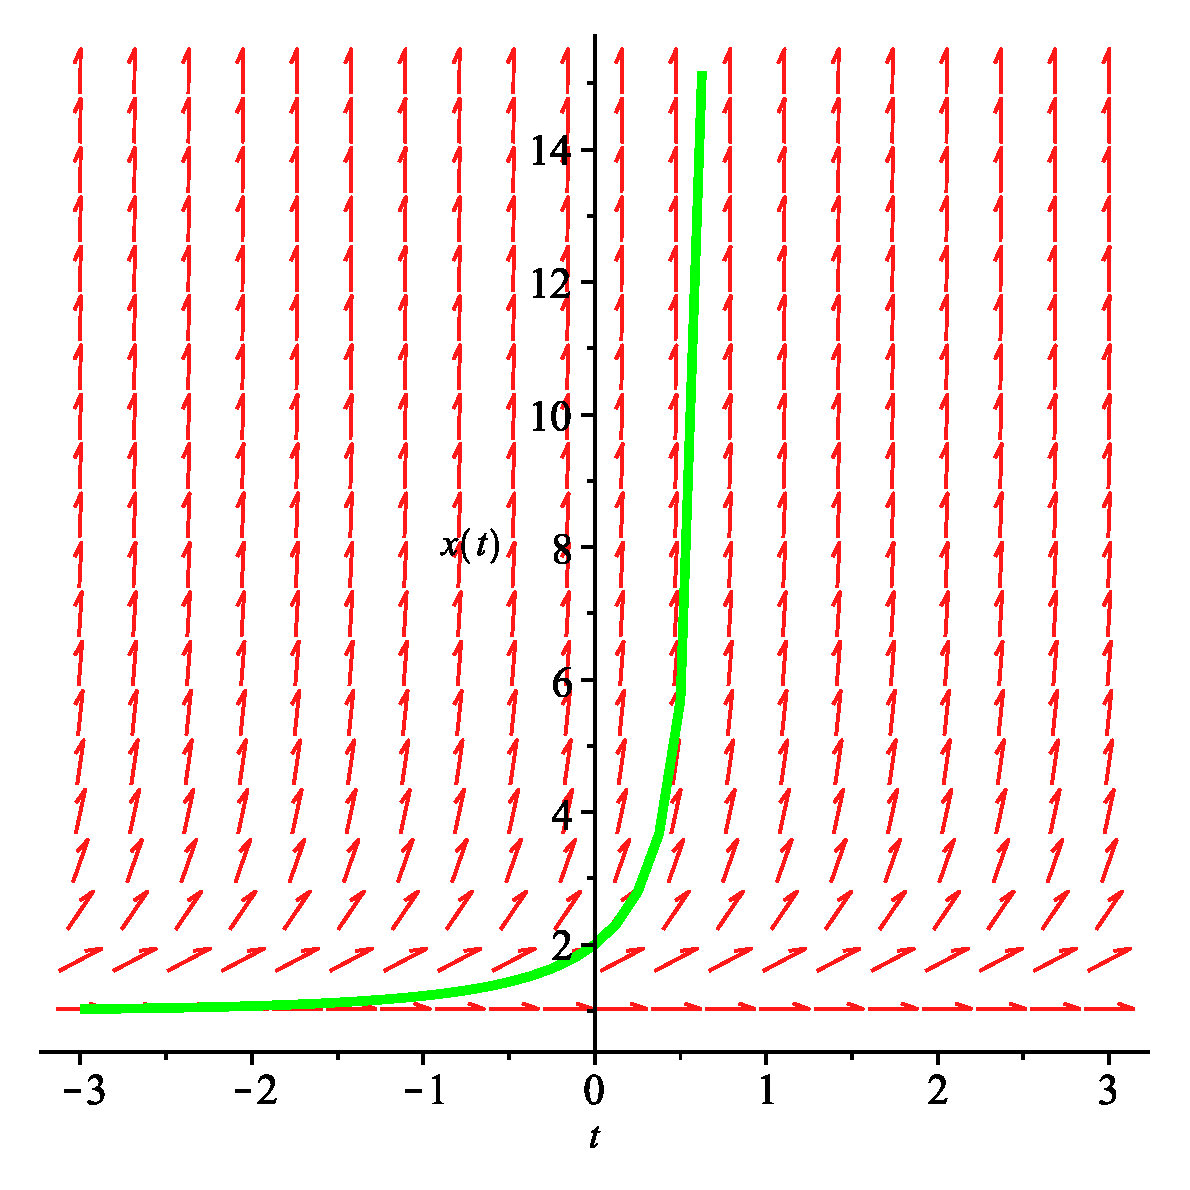
\includegraphics[width=10cm]{PortretEVS.eps}
\end{figure}

\subsection{Conclusions}
The section introduced the general method of solving equations with separable variables, presented in the classic differential equations books mentioned in the bibliography. The author's contribution were the selection and solving of the examples.




\section{Linear Differential Equations of First Order}

The following section introduces the reader to the general method of solving Linear Differential Equations of First Order, the solving method used in practice and a few examples.

\subsection{The General Form of a linear differential equation of first order}

A Linear differential equation has the following expression:

\begin{equation}
 x'=a(t)x+b(t) \label{LE} \tag{LE}
\end{equation}

where $a,b: (t_1,t_2) \subset \R\rightarrow\R$ are continous on $(t_1,t_2)$ (bounded or not). If $x=x(t)$, $t_1<t<t_2$ is a solutions for \eqref{LE}, then
multiplying with $exp(-\int_{t_0}^{t} a(s)ds)$, where $t_0$ is arbitrary chosen from $(t_1,t_2)$, the following equation is obtained
\begin{equation*}
 \frac{d}{dt}\bigg[ e^{-\int_{t_0}^{t} a(s)ds}x(t)\bigg] = b(t)e^{-\int_{t_0}^{t} a(s)ds}, t \in (t_1,t_2) 
\end{equation*}

So

\begin{equation}
 x(t)=e^{\int_{t_0}^{t} a(s)ds}x_0 + \int_{t_0}^{t} b(s)e^{-\int_{t_0}^{s} a(\sigma)d\sigma}ds , t \in (t_1,t_2) \label{SOL} \tag{SOL}
\end{equation}

where $x_0$ is an arbitrary real number. Reciprocally, we can easily agree that any function $x=x(t), t\in (t_1,t_2)$ given by the formula \eqref{SOL} is a solution for \eqref{LE}.
Actually, \eqref{SOL} asserts the solution of \eqref{LE} with the Cauchy condition $x(t_0)=x_0$.

Sometimes, it is more convienent to use the following form of \eqref{SOL}:

\begin{equation}
 x(t)= e^{\int a(s)ds}\cdot\int b(t)e^{-\int a(t) dt}dt \label{SOL*}\tag{SOL*}
\end{equation}

with the convention that $\int a(t) dt$ is a fixed primitive of $a=a(t)$ (the same in \eqref{SOL} and \eqref{SOL*}).

In practice, a method that does not require the use of \eqref{SOL} formula is based on the algebraic link which exists between the set of the \eqref{LE} solutions and the set of the associated homogeneous equation solutions: $$x'=a(t)x.$$
This link is contained in the following theorem:
\begin{theorem}\label{1.2.1.1}
 If $x_{p}$ is a particular solution of \eqref{LE}, than any other solution $x$ of the equation is the sum between a certain solution $x_{o}$ of the homogeneous equation and $x_{p}$, meaning: $$x=x_{o}+x_{p}.$$ Reciprocically, any solution $x_{o}$ of the homogeneous equation is the difference between a certain solution $x$ of \eqref{LE} and $x_{p}$.
\end{theorem}
The theorem sustains that for solving a \eqref{LE}, we have to go through two stages:
\begin{enumerate}
 \item to solve the associated homogeneous equation;
 \item to determine a particular solution of \eqref{LE}.
\end{enumerate}

\subsection{Examples}
$1)$ $x'+x\tan t=\frac{1}{\cos{t}}$, $t\in (-\frac{\pi}{2},\frac{\pi}{2})$\\\\
\underline{Solution}: For solving this equation, we will use the result from \ref{1.2.1.1}. 
The associated homogeneous equation is: $$x{o}'=-x_{o}\tan t.$$ Separating the variables, we get: $$\frac{dx_{o}}{x_{o}}=-\tan t dt.$$ By integration, we obtain: $$\ln{x_{o}}=\ln{\cos{t}}+c_{1},c_{1}\in\R \Leftrightarrow$$
$$x_{o}=c\cos{t}, c\in\R.$$ 
The particular solution for the given linear differential equation of first order is:
$$x_{p}=c(t)\cos{t}.$$ By replacing in the given equation, we obtain:
$$c'(t)\cos{t}-c(t)\sin{t}+c(t)\tan t\cos{t}=\frac{1}{\cos{t}}\Leftrightarrow$$
$$c'(t)\cos{t}=\frac{1}{\cos{t}}\Leftrightarrow$$
$$c'(t)=\frac{1}{\cos^{2}{t}}\Leftrightarrow$$
$$c(t)=\tan t.$$
Meaning that the particular solution is:
$$x_{p}=\tan t \cos{t} \Leftrightarrow x_{p}=\sin{t}.$$
Hence, the solution is:
$$x=x_{p}+x_{o} \Leftrightarrow x=\sin{t}+c\cos{t}.$$
$2)$ $\begin{cases}
       x'+x=e^{2t}\\
       x(0)=1
      \end{cases}$\\\\
      \underline{Solution:} The associated homogeneous equation is: $$x_{o}'=-x_{o}.$$ Separating the variables, we get: $$\frac{dx_{o}}{x_{o}}=-dt.$$ By integration, we obtain: $$\ln{x_{o}}=-t+c_{1},c_{1}\in\R\Leftrightarrow$$ 
      $$x_{o}=ce^{-t},c\in\R.$$ Hence, the particular solution for the given linear differential quation of first order has the following form: $$x_{p}=c(t)e^{-t}.$$ Further, replacing in the given equation we get: $$c'(t)e^{-t}-e^{-t}c(t)+e^{-t}c(t)=e^{2t}\Leftrightarrow$$
      $$c'(t)=e^{3t}\Leftrightarrow c(t)=\frac{1}{3}e^{3t}.$$
      Thus, the general solution has the following form:
      $$x=ce^{-t}+\frac{1}{3}e^{2t}, c\in \R.$$
      Then, by attaching the Cauchy condition, we get that the constant $c=\frac{2}{3}$, which means that the solution for the given Cauchy problem is: $$x=\frac{2}{3}e^{-t}+\frac{1}{3}e^{2t}.$$

\subsection{Conclusions}
The section introduced the notion of linear differential equation of first order and two methods of solving it, including the one used in practice, from the classic differential equations books mentioned in the bibliography. The author's contribution was the selection and solving of the examples. 
\section{Linear Differential Systems}
\subsection{The general form of a linear differential system}
Many evolutive processes from the real world can not be described by only one variable. Therefore, for two or more variables, we must consider a system 
of two or more differential equations. In the following chapter, we will consider differential systems of the first order:
\begin{equation}
\begin{cases}
 x'=f(t,x,y)\\ 
 y'=g(t,x,y)\\
\end{cases}
 \label{DS}\tag{DS}
\end{equation}

where $f$,$g$ are given functions and the unknowns are the functions $x,y$ of variable $t$. \\

\begin{definition} 
A solution for \eqref{DS} is a pair $(x,y)\in C^{1}(J)$, where $J\subseteq \R$, which satisfy on $J$ the two equations from \eqref{DS}, for 
any $t\in J$. 
\end{definition}
 
\eqref{DS} is linear if functions $f$ and $g$ depend affinely on $x$ and $y$. Then \eqref{DS} has the following form:
\begin{equation}
 \begin{cases}
  x'=a_{11}(t)x+a_{12}(t)y+b_{1}(t)\\
  y'=a_{21}(t)x+a_{22}(t)y+b_{2}(t)\\
 \end{cases}
\label{DS*}\tag{DS*}
\end{equation}

Coefficients $a_{ij}$ and free terms $b_{i}$ are alleged to be continuous functions on an interval $J$. If, in particular, coefficients $a_{ij}$
are constants, we say that the linear system is with constant coefficients. If $b_{i}=0$, we say that the system is homogeneous. If both situations
take place, the system is linear and homogeneous, with constant coefficients.

\subsection{Matrix Analysis Theory}

Let us define $\mathcal{M}_{nm}(\mathbb{K})$ the set of matrices with n rows and m columns, with elements from the field $\mathbb{K} (\R$ or $\mathbb{C})$. It is known that $(\mathcal{M}_{nm}(\mathbb{K}), +, \cdot, \R)$ is a linear space of dimension $n\cdot m$. It can be organized as a normalized space using the following norm:
\begin{equation*}
 \rVert A \rVert = \bigg( \sum_{i,j=1}^{n} a_{ij}^{2} \bigg)^\frac{1}{2}
\end{equation*}

Then $(\mathcal{M}_{nm}(\mathbb{K}), \rVert \cdot \rVert)$ is a Banach space. The defined norm has the following properties on the Banach space presented earlier:
\begin{enumerate}
  \item $\rVert A+B \rVert \leq \rVert A \rVert + \rVert B \rVert$
  \item $\rVert \lambda A \rVert = |\lambda|\rVert A \rVert$
  \item $\rVert Ax\rVert_{\R ^{n}} = \rVert A \rVert \rVert x \rVert _{\R ^{n}}$
  \item $\rVert A \cdot B \rVert \leq \rVert A \rVert \cdot \rVert B \rVert$
 \end{enumerate}
Next, let $M\in\mathcal{M}_{nn}(\mathbb{K})$. Then:
\begin{equation}
 e^{M}=\sum_{k\geq0} \frac{1}{k!} M^{k} \label{3.1} \tag{3.1}
\end{equation}
\begin{proof}
 Let $S_{n}=\sum_{k=0}^{n}\frac{1}{k!}M^{k}$ the partial sum of serie \eqref{3.1}. Next, we prove that $S_{n}$ is a Cauchy sequence in the Banach space $(\mathcal{M}_{nm}(\mathbb{K}), \rVert \cdot \rVert)$. 
 \begin{equation*}
  \rVert S_{n+p}-S_{n}\rVert=\rVert\frac{1}{(n+1!)} A^{n+1}+...+\frac{1}{(n+p!)} A^{n+p}\rVert
  \end{equation*}
  \begin{equation*}
   \leq \frac{1}{(n+1)!}\rVert A^{n+1}\rVert+...+\frac{1}{(n+p)!}\rVert A^{n+p}\rVert=|a_{n+p}-a_{n}|
  \end{equation*}
where $$a_{n}=\sum_{k=0}^{n}\frac{1}{k!}\rVert M \rVert ^{k}.$$\\
Due to the fact that $$\sum_{k\geq 0} \frac{1}{k!}x^{k}$$ is a convergent series and the sum of it is equal to $e^{x}$, $\forall x\in \R$ $\Rightarrow$ $$\sum_{k\geq 0}\frac{1}{k!}\rVert M \rVert ^{k}$$ is convergent, therefore $a_{n}$ is convergent, which means that $a_{n}$ is Cauchy $\Rightarrow$ $\forall \varepsilon > 0$,  $\exists n(\varepsilon) \in \mathbb{N}$ so that $$\rVert S_{n+p} - S_{n} \rVert \leq \varepsilon$$ $\forall n\geq n(\varepsilon)$, $ \forall p\in \mathbb{N}$ $\Rightarrow$ $(S_{n})$ is a Cauchy sequence $\Rightarrow$ the existence of \eqref{3.1} is proved.


\end{proof}





\subsection{Existence and uniqueness theorems}

Let us consider the system:
\begin{equation}
 \begin{cases}
  u'=A(t)u+B(t)\\
u(t_{0})=u_{0}
 \end{cases}\label{Sys1}\tag{Sys1}
\end{equation}

where $t\in J=[t_{0}-a,t_{0}+a], a>0$ $t_{0}\in J$ and $u_{0}\in\R^{2}$. \newline
Regarding the existence and uniqueness of the solution of the previous system, we present the following result:
\begin{theorem}
 Considering \eqref{Sys1}, we assume that $A\in C(J,\mathcal{M}_{2}(\R))$, $B\in C(J,\R^{2})$. Then, there exists a unique 
 solution $u^{*}\in C^{1}(J,\R^{2})$.
\end{theorem}
\begin{proof}
 We will use the following Lemma:
 \begin{lemma}
  The solution $u^{*}$ is equivalent to the following system of integral equations:
  \begin{equation}
   u(t)=\int_{t_0}^{t}\bigg[ A(s)u(s)+B(s)\bigg] ds+u_{0} \label{IntSol}\tag{IntSol}
  \end{equation}
 \end{lemma}
\begin{proof}
  \textquotedblleft $\Rightarrow$ \textquotedblright
  If $u$ satisfies \eqref{Sys1}, then by integrating from $t_{0}$ to $t\in J$, we get:
  \begin{equation*}
   u(t)-u(t_{0})=\int_{t_0}^{t}\bigg[ A(s)u(s)+B(s)\bigg] ds
  \end{equation*}
$u(t_{0})=u_{0}$ $\Rightarrow$ \eqref{IntSol}.\newline
\textquotedblleft$\Rightarrow $\textquotedblright
  Let $u$ be a solution of \eqref{IntSol}. Then $u'(t)=A(t)u+B(t)$. Since the right side is continuous, we obtain that $u\in C^{1}(J,\R)$.
  Moreover, $u(t_{0})=u_0$.
  The lemma is proved.
\end{proof}
Resuming the proof of the theorem, let us denote $A:C(J,\R^{2})\rightarrow C(J,\R^{2})$, $u\longmapsto Au$, where:
$Au(t):=\int_{t_0}^{t}\bigg[ A(s)u(s)+B(s)\bigg] ds+u_{0}$

\textquotedblleft\eqref{IntSol} $\Leftrightarrow$ $u=Au$\textquotedblright

We consider on $C(J,\R^2)$ the Bielecki norm:
\begin{equation*}
\Arrowvert u \Arrowvert_{B} = max_{t\in J}(\Arrowvert u \Arrowvert_{\R^2} e^{-\tau\arrowvert t-t_{0}\arrowvert}), \tau>0
\end{equation*}
$(C(J,\R^{2}),\Arrowvert\ldotp\Arrowvert)$ is a Banach space.\newline
Then we have that $\Arrowvert Au-Av\Arrowvert_{B}\leq L_{A} \Arrowvert u-v \Arrowvert_{B}, \forall u,v \in C(J,\R^{2}, L_{A} \in (0,1))$.\newline
For $t\geq t_{0}$:\\


 $$\Arrowvert Au(t)-Av(t) \Arrowvert _ {\R^{2}} = \Arrowvert \int_{t_{0}}^{t} A(s)(u(s)-v(s)) ds \Arrowvert$$ 
 $$\leq \int_{t_{0}}^{t} \Arrowvert A(s)(u(s)-v(s)) \Arrowvert ds$$ 
 $$\leq \int_{t_{0}}^{t} \Arrowvert A(s) \Arrowvert _ {\M(\R^{2})} \Arrowvert u(s)-v(s) \Arrowvert _ {\R^{2}}ds$$
 $$\leq M_{A} \int_{t_{0}}^{t} \Arrowvert u(s)-v(s) \Arrowvert e^{-\tau(s-t_{0})}e^{\tau(s-t_{0})} ds$$
 $$\leq \int_{t_{0}}^{t} \smash{\displaystyle\max_{(s \in J)}} (\Arrowvert u(s)-v(s)\Arrowvert  e^{-\tau(s-t_{0})})  e^{\tau(s-t_{0})} ds $$
 $$\leq M_{A} \Arrowvert u-v \Arrowvert _ {B} \frac{1}{\tau}(e^{\tau(t-t_{0})}-1)$$
 $$\leq \frac{M_{A}}{\tau} \Arrowvert u-v \Arrowvert _ {B} e^{\tau(t-t_{0})}$$ 
 $$\Rightarrow \Arrowvert Au-Av \Arrowvert \leq \frac{M_{A}}{\tau} \Arrowvert u-v \Arrowvert _ {B}.$$ Let $L_{A}=\frac{M_{A}}{\tau}$ such as $\tau > M_{A}$. Then $L_{A}<1$.



\end{proof}






\subsection{Representations of the solution}

Let us remark that \eqref{DS} can be written as a single vectorial equation:
\begin{equation}
 u'=F(t,u) \label{VDS}\tag{VDS}
\end{equation}
where $u$ and $F$ are vectorials, with two real components, more exactly column matrix:\newline
\begin{equation*}
u =
 \begin{bmatrix}
  x\\
  y\\
 \end{bmatrix}
, \quad F(t,u) =
\begin{bmatrix}
 f(t,x,y)\\
 g(t,x,y)\\
\end{bmatrix}
\end{equation*}
\newline

The condition for the Cauchy Problem of the system can be written:
\begin{equation*}
 u(t_{0})=u_{0},\\
 u_{0}= \begin{bmatrix}
         x_{0}\\
         y_{0}
        \end{bmatrix}
\end{equation*}
\newline
Also, \eqref{DS*} can be written:
\begin{equation}
 u'=A(t)u+B(t) \label{MDS}\tag{MDS}
\end{equation}
where 
\begin{equation*}
 A(t)=\begin{bmatrix}
       a_{11}(t) & a_{12}(t)\\
       a_{21}(t) & a_{22}(t)\\
      \end{bmatrix}
\quad
B(t)=\begin{bmatrix}
      b_{1}(t)\\
      b_{2}(t)
     \end{bmatrix}
\end{equation*}

\begin{theorem}[of representing the solutions of linear systems]
 Let $A\in C(J,\mathcal{M_{2}}))$ and $B\in(J,R^{2})$. Then the solutions of the linear system \eqref{MDS} are defined by the formula 
 \begin{equation}\label{1.2}
  u=e^{\int_{t_0}^{t} A(\sigma)d\sigma}C+\int_{t_0}^{t}e^{\int_{s}^{t} A(\sigma)d\sigma}B(s)ds
 \end{equation}
where $C=\begin{bmatrix}C_{1}\\ C_{2}\end{bmatrix}$ and $C_{1}, C_{2}\in \R.$

\end{theorem}

\begin{theorem}[of existence, uniqueness and representation of the solution]
 Let $A\in C(J,M_{2}(\R)), B\in C(J,\R), t_{0}\in J and u_{0}\in \R^{2}$. Then the Cauchy Problem has a unique solution 
 defined on $J$, given by the formula:
 \begin{equation}\label{1.3}
  u=e^{\int_{t_0}^{t} A(\sigma)d\sigma}u_{0}+\int_{t_0}^{t}e^{\int_{s}^{t} A(\sigma)d\sigma}B(s)ds
 \end{equation}

\end{theorem}

\begin{theorem}[the structure of the set of solutions]

(a) The set of solutions of a bidimensional linear and homogeneous system is a linear bidimensional space.\\
(b) If $u_{p}$ is a particular solution of a linear non-homogeneous system \eqref{MDS}, then any other solution $u$ of the system \eqref{MDS}
is the sum between the solution of the homogeneous system ($u_{o}$) with the particular solution $u_{p}$:
\begin{equation*}
 u=u_{o}+u_{p}
\end{equation*}
\end{theorem}

\begin{definition}
 A matrix in which the columns are the linearly independent solutions of the homogeneous system is called fundamental matrix of the system.
\end{definition}
 
 \begin{lemma}\label{1.3.4.4.}
  (a) Any fundamental matrix is unsingular for any $t \in J$.\\
  (b) Any fundamental matrix $U(t)$ satisfies the differential matricial equation:
  \begin{equation*}
   U'(t)=A(t)U(t)
  \end{equation*}

 \end{lemma}
\subsection{Representation with fundamental matrix}
In this paragraph, let us submit the possibility of representing the solutions of the non-homogeneous system in terms of the fundamental matrix $U(t)$, of which purpose is to replace the matrix $e^{\int_{t_{0}}^{t} A(\sigma)d\sigma}$ from \eqref{1.2}.\\
Firstly, let $$u_{p}=U(t)C(t)$$ be a particular solution of the non-homogeneous system, where the vectorial function $$C(t)=
\begin{bmatrix}
 C_{1}(t)\\
 C_{2}(t)
\end{bmatrix}$$ is to be determined with the condition that $u_{p}$ satisfies the given system. Hence
$$u'_{p}=U'(t)C(t)U(t)C'(t)$$
and by replacing we find that
$$U'(t)C(t)+U(t)C'(t)=A(t)U(t)C(t)+B(t).$$
Point $b)$ from lemma \ref{1.3.4.4.} guarantees that
$$U'(t)=A(t)U(t).$$
Thus $U(t)C'(t)=B(t)$, which means that $C'(t)=U^{-1}(t)B(t)$. Then, according to point $a)$ from \ref{1.3.4.4.}, matrix $U(t)$ is invertible. Let us choose
$$C(t)=\int_{t_0}^{t} U^{-1}(s)B(s)ds$$
and so we get a particular solution of the non-homogeneous system:
$$u_{p}=\int_{t_0}^{t} U(t)U^{-1}(s)B(s)ds.$$
Thus, an equivalent of \eqref{1.2} is:
\begin{equation}\label{1.4}
 u=U(t)C+\int_{t_0}^{t} U(t)U^{-1}(s)B(s)ds.
\end{equation}
The analogue of \eqref{1.3} results immediately:
\begin{equation}\label{1.5}
 u=U(t)U^{-1}(t_{0})u_{0}+\int_{t_0}^{t} U(t)U^{-1}(s)B(s)ds.
\end{equation}

Hence, we can present the following theorem:
\begin{theorem}[of representation with fundamental matrix]\label{1.3.5.1}
 If $U(t)$ is a fundamental matrix of \eqref{MDS}, then:
 \begin{enumerate}[(i)]
  \item The solutions of the homogeneous system are the functions $u_{o}=U(t)C$, where $C$ is a random vector from $\R^{2}$;
  \item The solutions of the non-homogeneous system are the functions defined by \eqref{1.4}, where $C\in\R^{2}$;
  \item The solution of the Cauchy problem for \eqref{Sys1} is the function defined by formula \eqref{1.5}.
 \end{enumerate}
\end{theorem}
According to \ref{1.3.5.1}, solving a linear system depends on finding a fundamental matrix. Generally, this is not possible, but for the systems with constant coefficients is possible.


\subsection{Linear systems with constant coefficients}

In this paragraph, we consider the system \eqref{DS*}, where the coefficients $a_{ij}(i,j=1,2)$ are constant, and $b_{1},b_{2}\in C(J)$. By using matrices, we can rewrite the system as:
$$u'=Au+B(t),$$
where
$$u=\begin{bmatrix}
     x\\
     y\\
    \end{bmatrix}, 
A=\begin{bmatrix}
   a_{11} & a_{12}\\
   a_{21} & a_{22}\\
  \end{bmatrix},
B=\begin{bmatrix}
   b_{1}(t)\\
   b_{2}(t)\\
  \end{bmatrix}.$$

Due to the fact that all the previous results stay valid, the solutions of the system have the following form:
$$u=u_{o}+u_{p}.$$
The explicit form of the solution is:
\begin{equation*}
 u=e^{(t-t_{0})\cdot A}\cdot C+\int_{t_0}^{t} e^{(t-s)\cdot A}B(s) ds,
\end{equation*}
where the constant vector $C$ is random. Also, the Cauchy problem, with $u(t_{0})=u_{0}$ as the initial condition admits only one solution, which is
\begin{equation}\label{1.6}
  u=e^{(t-t_{0})\cdot A}\cdot u_{0}+\int_{t_0}^{t} e^{(t-s)\cdot A}B(s) ds
\end{equation}
If by the replacement of $e^{(t-t_{0})\cdot A}$ it is considered another fundamental matrix $U(t)$, then the solutions of the system and also for the Cauchy problem are given by formulas \eqref{1.4} and \eqref{1.5}. The question of how we can determinate the fundamental matrix and how we can directly solve the system still remains.\\
For this, let us search for solutions for the associated homogeneous system based on the following form:
$$u=e^{rt}V,$$
where $r\in\R$ and $V=\begin{bmatrix} v_{1}\\v_{2}\\ \end{bmatrix} \in \R^{2}$ are determined with the condition that $u$ satisfies the homogeneous system. Obviously, $V\neq 0$. By replacing in the homogeneous system, we get:
$$re^{rt}V=A(e^{rt}V)=e^{rt}AV.$$
By simplifying with $e^{rt}$, we obtain:
\begin{equation}\label{1.7}(A-rI)V=0.\end{equation}
As $V\neq 0$, we conclude that $r$ is an eagen value of matrix $A$, and $V$ is an eagen vector associated to this value. Eagen values are determined with the condition that the algebraic homogeneous system \eqref{1.7} admits solutions unequal to $0$, meaning from equation:
\begin{equation}\label{1.8}
 det(A-rI)=0.
\end{equation}
This equation is named the characteristic equation of the system and is a second grade polynomial. It can be written:
\begin{equation}
 \begin{vmatrix}\label{det}
 a_{11}-r & a_{12}\\
 a_{21} & a_{22}-r\\
\end{vmatrix}
=0,
\end{equation}
where, by solving the determinant, we obtain:
$$r^{2}-(a_{11}+a_{22})r+a_{11}a_{22}-a_{12}a_{21}=0,$$
meaning
$$r^{2}-(tr A)r+det A=0.$$
Here, $$tr A=\sum_{i=0}^{n}a_{ii}$$ is the trace of the matrix. Considering how the roots of the characteristic equations might be, we distinguish the following cases:
\subsubsection{Case of real and distinct roots}
Let $r_{1},r_{2}$ be the roots of the characteristic equation, which are presumed to be real and distinct.
For each one, we choose a non-null solution of system \eqref{1.7}. Let them be $V_{1},V_{2}$. Meaning that we obtained two solutions for the homogeneous system:
$$ u_{1}=e^{r_{1}t}V_{1},\quad u_{2}=e^{r_{2}t}V_{2}.$$
As $r_{1}\neq r_{2}$, they are linear independent. Matrix $U(t)$, with columns $u_{1},u_{2}$ thus determined, is a fundamental matrix.

\subsubsection{Case of equal roots}
Let us presume that the roots of the characteristic equation are equal. Then $r:=r_{1}=r_{2}=\frac{tr A}{2}$. A solution of the system can be determined similarly to the previous case, of form $u_{1}=e^{rt}V$, where $V$ is a non-null solution of the algebraic homogeneous system \eqref{1.7}. A second solution $u_{2}$, linear independent of $u_{1}$, is searched by the form $u_{2}=e^{rt}(tV+W)$, with $V$ being the previous, and $W$ being vector which is obtained with the condition that verifies the system. We have:
$$ u'_{2}=re^{rt}(tV+W)+e^{rt}V$$
meaning that $u_{2}$ is a solution if
$$re^{rt}(tV+W)+e^{rt}V=e^{rt}A(tV+W).$$
By simplifying with $e^{rt}$ and by reducing the equal terms, we obtain the following algebraic linear and non-homogeneous system:
$$(A-rI)W=V.$$
This system is compatible and so we can choose a solution $W$ of it.

\subsubsection{Case of complex roots}
Let us presume that the roots of the characteristic equation are complex, being them $\alpha \pm \beta i$. Considering one of them, for example $\alpha + \beta i$ and by proceeding like in the case of real and distinct roots, let us determine a solution of the system, this time complex:

 $$u=e^{rt}V=e^{(\alpha+\beta i)t}(V_{1}+iV_{2})=
 e^{\alpha t}(\cos{\beta t}+i\sin{\beta t})(V_{1}+iV_{2})=$$
 $$=e^{\alpha t}[V_{1}\cos{\beta t}-V_{2}\sin{\beta t}+i(V_{1}\sin{\beta t}+V_{2}\cos{\beta t})].$$

where $V_{1},V_{2}$ represents the column vector of the real parts, respectively the coefficients of the imaginary parts of $V$, meaning $V=V_{1}+iV_{2}$ and $V_{1},V_{2} \in \R^{2}$. 
With the system being linear, homogeneous and with real coefficients, at once with a complex solution $u$, admits as solutions the conjugate function $\bar{u}$, as well as any linear combination of theirs with complex coefficients, particularly the real functions:
$$u_{1}:=Re (u)=\frac{1}{2}(u+\bar{u})=e^{\alpha t}(V_{1}\cos{\beta t}-V_{2}\sin{\beta t}),$$
$$u_{2}:=Im (u)=\frac{1}{2i}(u-\bar{u})=e^{\alpha t}(V_{1}\sin{\beta t}+V_{2}\cos{\beta t}).$$
 
 \subsection{Examples}
 $1)$ 
 $U'=AU$, where $A=\begin{bmatrix}
                    0 && 4\\
                    5 && 1\\
                   \end{bmatrix}$, $U=\begin{bmatrix} u_{1} \\ u_{2}\end{bmatrix}$.
                   
 \underline{Solution:}
First, let us attach the characteristic equation: $r^{2}-(tr(A))r+det(A)=0$. In our case, $tr(A)=1$ and $det(A)=-20$, meaning that the equation becomes: $r^{2}-r-20=0$. By solving the equation, we get the following roots: $r=5$ and $r=-4$. 
Let us consider the first case, where $r=5$. Next, we need to determine an eigenvector $V=\begin{bmatrix}
                                                                                           v_{1}\\
                                                                                           v_{2}
                                                                                          \end{bmatrix}$,by solving $(A-rI)V=0$. A convienent eigenvector would be $V=\begin{bmatrix}
                                                                                          4\\
                                                                                          -5\\\end{bmatrix}$
Hence, the solution is:
$$ U_{1}=e^{rt}V=e^{5t}\begin{bmatrix}4\\-5\\\end{bmatrix}=\begin{bmatrix} 4e^{5t} \\ -5e^{5t} \end{bmatrix}.$$
                                                            
                                                            
Next, we consider the case where $r=-4$. Thus, an eigenvector would be $V=\begin{bmatrix} 1 \\ -1 \end{bmatrix}$. Hence, the solution is:
$$U_{2}=e^{-4t}\begin{bmatrix} 1 \\ -1 \end{bmatrix}=\begin{bmatrix} e^{-4t}\\-e^{-4t}\end{bmatrix}.$$

Then, the fundamental matrix of the solutions of the system is:

$$U=c_{1}U_{1}+c_{2}U_{2},$$
where $c_{1},c_{2} \in \R$.

                                                                                    
$2)$ $U'=AU$, where $A=\begin{bmatrix}
                    -3 && -8\\
                    2 && 5\\
                   \end{bmatrix}$, $U=\begin{bmatrix} u_{1} \\ u_{2}\end{bmatrix}$.\\
\underline{Solution:}
By attaching the characteristic equation, we get that $r=1$ is a solution of the equation of multiplicity 2. We are in the case of equal roots. Next, by solving the equation $(A-rI)V=0$, we get that $V=\begin{bmatrix} -2\\1\end{bmatrix}$ is an eigenvector of the given equation. By solving $(A-rI)W=V$, we get $W=\begin{bmatrix} 1\\ -\frac{2}{8} \end{bmatrix}$. Then:
$$ U_{1}=e^{t}\begin{bmatrix} -2\\1\end{bmatrix}$$ and $$U_{2}=e^{t}\begin{bmatrix} -2t+1\\t-\frac{2}{8} \end{bmatrix}.$$
Hence, the fundamental matrix of the solutions has is $U=c_1U_{1}+c_{2}U_{2}$, where $c_{1},c_{2} \in \R$.

$3)$ $U'=AU$, where $A=\begin{bmatrix}
                    5 && 5\\
                    -4 && 3\\
                   \end{bmatrix}$, $U=\begin{bmatrix} u_{1} \\ u_{2}\end{bmatrix}$.\\
    \underline{Solution:}
    By solving the characteristic equation, we denote that we are in the case of complex roots, where $r=1\pm2i$. Next, we find that $V=\begin{bmatrix} 1 \\ -\frac{4}{5}+i\frac{2}{5} \end{bmatrix}$ is a convienient eigenvector for the case. The solution is 
    $$ U=e^{(1+2i)t}\begin{bmatrix} 1 \\ -\frac{4}{5}+i\frac{2}{5} \end{bmatrix} 
    = e^{t}(\cos{2t}+i\sin{2t})\bigg( \begin{bmatrix} 1\\ -\frac{4}{5}\end{bmatrix} + \begin{bmatrix} 0\\ \frac{2}{5}\end{bmatrix} i \bigg).$$
    By separating the real part and the imaginary part, we get two real solutions:
    $$U_{1}=e^{t}\bigg( \cos{2t}  \begin{bmatrix} 1\\ -\frac{4}{5}\end{bmatrix} - \sin{2t} \begin{bmatrix} 0\\ \frac{2}{5}\end{bmatrix} \bigg) $$ and
    $$ U_{2}=e^{t}\bigg( \cos{2t} \begin{bmatrix} 0\\ \frac{2}{5}\end{bmatrix} + \sin{2t} \begin{bmatrix} 1\\ -\frac{4}{5}\end{bmatrix} \bigg).$$
    
    \subsection{Conclusions}
    The section introduced the general form of linear systems with differential equations, the existence and uniqueness of the solution and its representations. Moreover, there were presented the three cases of linear systems with constant coefficients and examples. The author's contribution were the selection and solving of the examples.
    
    
    \chapter{Difference Equations}
    \section{Linear difference equations of first order}
    The general form of a linear difference equation of first order is:
    \begin{equation} 
     x_{n+1}=a_{n}x_{n}+b_{n} \label{2.1}
    \end{equation}
    for any $n \geq 0$, where $(a_{n})_{n\geq 0}$ and $(b_{n})_{n\geq 0}$ are given series of real numbers. 
\eqref{2.1} is obtained starting from an initial value $x_{0} \in \R$. Hence:
\begin{align*}
 x_{1} & =a_{0}x_{0}+b_{0}\\
   x_{2} & =a_{1}x_{1}+b_{1} = a_{1}(a_{0}x_{0}+b_{0})+b_{1}\\
  & = a_{1}a_{0}x_{0}+a_{1}+b_{0}+b_{1}\\
  & ...\\
   x_{n}&=a_{n-1}x_{n-1}+b_{n-1} = a_{n-1}\cdot ... \cdot a_{0}x_{0}+a_{n-1}\cdot ...\cdot a_{1}b_{0}+...+a_{n-1}\cdot b_{n-2}+b_{n-1}.
\end{align*}

Through mathematical induction, it is proved that the solution of the linear difference equation of first order has the following form:
\begin{equation}\label{2.2}
 x_{n}=\bigg( \prod_{j=0}^{n-1} a_{j} \bigg) \cdot x_{0} + \sum_{j=0}^{n-1} \bigg( \prod_{k=j+1}^{n-1} a_{k} \bigg)\cdot b_{j}.
\end{equation}
If \eqref{2.1} is valid for $n$ starting from an $n_{0} \geq 0$, meaning that:
\begin{equation}\label{2.3}
 x_{n+1}=a_{n}\cdot x_{n}+b_{n}, n\geq n_{0}
\end{equation}
Then \eqref{2.2} becomes:
\begin{equation}
 x_{n}=\bigg( \prod_{j=n_{0}}^{n-1} a_{j} \bigg) \cdot x_{n_{0}} + \sum_{j=n_{0}}^{n-1} \bigg( \prod_{k=j+1}^{n-1} a_{k} \bigg)\cdot b_{j}.
\end{equation}
Ordinarilly, there are multiple particular cases of \eqref{2.1} that can appear in practice, which ease the use of formula \eqref{2.2}.
\subsection{Particular cases of \eqref{2.1}}
\subsubsection{Case $a_{n}\equiv a$} \label{i}
In this case, \eqref{2.1} becomes:
\begin{equation}
\label{2.6}
 x_{n+1}=a\cdot x_{n}+b_{n}, n\geq 0,
\end{equation}
where $a\in \R$ and $(b_{n})_{n\in\mathbb{N}}$ is a given series of real numbers.
From \eqref{2.1} we have that:
\begin{align*}
 \prod_{j=0}^{n-1} a_{j} &=\prod_{j=0}^{n-1} a,\\
 \prod_{k=j+1}^{n-1} a_{k}&=\prod_{k=j+1}^{n-1} a=a^{n-1-(j+1)+1}=a^{n-j-1}
\end{align*}
and the solution is:
\begin{equation}\eqref{2.6}
 x_{n}=a^{n}\cdot x_{0}+\sum_{j=0}^{n-1} a^{n-j-1}\cdot b_{j}.
\end{equation}

\subsubsection{Case $b_{n}\equiv b$}\label{2.1.1.2}
In this case, \eqref{2.1} becomes:
\begin{equation}\label{2.7}
 x_{n+1}=a_{n}\cdot x_{n}+b, n\geq 0,
\end{equation}
where $b\in\R$ and $(a_{n})_{n\in\mathbb{N}}$ is a given series of real numbers.
From \eqref{2.2}, we obtain:
\begin{align*}
 x_{n} &= \bigg( \prod_{j=0}^{n-1} a_{j} \bigg) \cdot x_{0} + \sum_{j=0}^{n-1}\bigg(\prod_{k=j+1}^{n-1} a_{k}\bigg)\cdot b_{j} =\\
 &= \bigg( \prod_{j=0}^{n-1} a_{j} \bigg) \cdot x_{0} + \sum_{j=0}^{n-1}\bigg(\prod_{k=j+1}^{n-1} a_{k}\bigg)\cdot b
\end{align*}
meaning that the solution is of form:
\begin{equation}
 x_{n}=\bigg( \prod_{j=0}^{n-1} a_{j} \bigg)\cdot x_{0}+b\cdot\sum_{j=0}^{n-1}\bigg(\prod_{k=j+1}^{n-1} a_{k}\bigg).
\end{equation}
\subsubsection{Case $a_{n}\equiv a$ and $b_{n}\equiv b$}
In this case, \eqref{2.1} becomes:
\begin{equation}
 x_{n+1}=a\cdot x_{n}+b, n\geq 0,
\end{equation}
where $a,b\in \R$.
From \eqref{2.2} we obtain:
\begin{align*}
 x_{n} &= \bigg(\prod_{j=0}^{n-1} a \bigg)\cdot x_{0}+\sum_{j=0}^{n-1}\bigg(\prod_{k=j+1}^{n-1}a\bigg)\cdot b=\\
 &=a^{n}\cdot x_{0}+b\cdot \sum_{j=0}^{n-1} a^{n-j-1}=\\
 &=a^{n}\cdot x_{0}+b\cdot (a^{n-1}+a^{n-2}+...+a^{0}).
\end{align*}
If $a \neq 1$, we have:
\begin{align*}
 x_{n}&=a^{n}\cdot x_{0}+b\cdot \frac{a^{n}-1}{a-1}=\\
 &= a^{n}\cdot \bigg(x_{0}+\frac{b}{a-1}\bigg)-\frac{b}{a-1}.
\end{align*}
And if $a=1$, we have:
\begin{align*}
 x_{n}&=a^{n}\cdot x_{0}+b(a^{n-1}+a^{n-2}+...+a^{0})=\\
 &=x_{0}+n\cdot b.
\end{align*}
Thus the solution is:

 $$x_{n}=\begin{cases}
        a^{n}\cdot \big(x_{0}+\frac{b}{a-1}\big)-\frac{b}{a-1}, a\neq 1 \\
        x_{0}+n\cdot b, a=1.
       \end{cases}
$$

\subsection{Examples}
$1)$ $x_{n+1}=-x_{n}+n$\\
\underline{Solution:}
In this example, $a_{n}=a=-1\in\R$, meaning we are in case \ref{i}. Then, the products become:
$$ \prod_{j=0}^{n-1} a=a^{n}=(-1)^{n}$$
and 
$$\prod_{k=j+1}^{n-1} a=(-1)^{n-j-1}.$$ 
Hence, by applying \eqref{2.6}, the solution is:
$$x_{n}=(-1)^{n}\cdot x_{0}+\sum_{j=0}^{n-1} (-1)^{n-j-1}\cdot j.$$
$2)$ $x_{n+1}=\frac{n+2}{n+1}\cdot x_{n}$.\\
\underline{Solution:}\\ \\
In this example, $a_{n}=\frac{n+2}{n+1}$ and $b_{n}=0 \in \R$, meaning we are in case \ref{2.1.1.2}. Then, the solution is:
$$ x_{n}=\prod_{j=0}^{n-1} \frac{j+2}{j+1}=\prod_{j=0}^{n-1} (1-\frac{1}{n+1})=(1-1)\cdot ...\cdot (1-\frac{1}{n})=0$$
\subsection{Conclusions}

\section{Dynamical systems}
\subsection{General notions}
$(G,+,\tau)$ is a topological semigroup if:
\begin{enumerate}[i)]
 \item $(G,+)$ is a semigroup;
 \item $(G,\tau)$ is a separate topological space;
 \item operator 
 $$ +:GxG\rightarrow G, (t_{1},t_{2})\longmapsto t_{1}+t_{2}$$ is continuous.
\end{enumerate}
Let $(X,d)$ be a metric space, $(G,+,\tau)$ a topological semigroup and $\varphi : GxX\rightarrow X$.
\begin{definition}The triplet $(X,G,\varphi)$ is called a dynamical system if:
\begin{enumerate}
 \item $\varphi(0,x)=x, \forall x\in X$;
 \item $\varphi(t, \varphi(s,x))=\varphi(t+s,x), \forall t,s\in G, \forall x\in X$;
 \item operator $\varphi$ is continuous.
\end{enumerate}
\end{definition}
Space $X$ is called phase space or states space. Operator $\varphi(+,\cdot):X\rightarrow X$, $t\in G$ is called the movement of x in relation to the dynamical system $(X,G,\varphi)$. The set $\varphi(G,x)$ is called the trajectory of $x$ or the trajectory of the dynamical system passing through x. If $(G,+)$ is a group, then the dynamical system is a discrete dynamical system, and if $G=\R$ then the dynamical system is continuous.
\subsection{Dynamical systems defined by a linear difference equation of first order}
\subsubsection{Example}\label{2.2.2.1} Let us consider the difference equation:
\begin{equation}
 x_{n+1}=ax_{n}, a\in \R^{*} \label{2.10}
\end{equation}
We know that $x_{n}=a^{n}x_{0}, x_{0}\in\R$ represents the solution of \eqref{2.10} with start value $x_{0}\in\R$. Let us define $\varphi:\mathbb{Z}x\R\rightarrow X$ through:
$$\varphi(k,x)=a^{k}x.$$
then $(\R,\mathbb{Z},\varphi)$ is an inversable discrete dynamical system generated by \eqref{2.10}.
\subsubsection{Example}\label{2.2.2.2}
Let $f:\R\rightarrow\R$ and the difference equation:
\begin{equation}\label{2.11}
 x_{n+1}=f(x_{n}).
\end{equation}
We note through
\begin{equation}\label{2.12}
 x_{n}(x_{0})=\underbrace{(f\circ...\circ f)}_\text{of n times}(x)=f^{n}(x_{0}), x_{0}\in\R
\end{equation}
the solution of the equation with start value $x_{0}\in\R$. We define $\varphi:\mathbb{N}x\R\rightarrow\R$ through:
\begin{equation*}
 \varphi(n,x)=f^{n}(x),
\end{equation*}
then $(\R,\mathbb{N},\varphi)$ is a discrete dynamical system generated by \eqref{2.11}. The trajectory of the dynamical system that passes through $x_{0}\in\R$ is given by the set:
\begin{equation}\label{2.13}
 \varphi(\mathbb{N},x_{0})=O_{f}(x_{0})=\{x_{0},x_{1},...,x_{n},...\}
\end{equation}
named also the orbit generated by $x$ through $f$.
\begin{definition}
 Let $(X,G,\varphi)$ be a dynamical system. We say that $\xstar\in X$ is a fixed point of the dynamical system if $\varphi(t,\xstar)=\xstar,\forall t\in G$.
\end{definition}
Let us consider the dynamical system generated by \eqref{2.11}. If $\xstar \in \R$ is a fixed point for this dynamical system, then:
\begin{align*}
 \varphi(n,\xstar)&=\xstar, \forall n\in\mathbb{N}\\
 f^{n}(\xstar)&=\xstar,\forall n\in\mathbb{N}
\end{align*}
from where we deduce that $\xstar\in\R$ is a solution for the equation $f(x)=x$. So the orbit generated by the fixed point $\xstar$ is reduced to a point
\begin{equation*}
 \varphi(\mathbb{N},\xstar)=O_{f}(\xstar)=\{\xstar\}.
\end{equation*}
\section{Dynamics generated by difference equations of first order}
\subsection{Equilibrium point. Stability criteria}
As we have seen in \ref{2.2.2.2}, the difference equation of first order:
\begin{equation}\label{2.14}
 x_{n+1}=f(x_{n})
\end{equation}
generates the dynamical system $(\R,\mathbb{N,\varphi})$, where $\varphi(n,x)=f^{n}(x)$. The fixed points of this dynamical system are given by the solutions of the equation
\begin{equation}\label{2.15}
 x=f(x)
\end{equation}
From the perspective of the difference equation \eqref{2.14}, the fixed points of the generated dynamical system are obtained from the constant solutions:
\begin{equation}\label{2.16}
(x_{n})=(\xstar,\xstar,...\xstar)
\end{equation}
where $\xstar\in\R$ is the solution of \eqref{2.15}.
\begin{definition}
 A point $\xstar\in\R$ is called an equilibrium point (stationary) for equation \eqref{2.14} if it is a fixed point for the generated dynamical system $(\R,\mathbb{N},\varphi)$. The constant solution defined by \eqref{2.16} is called equilibrium solution (stationary).
\end{definition}
One of the main objectives in the study of dynamics generated by difference equations is the study of the behaviour of their solutions to the equilibrium solutions. We will introduce the stability notions that describe this behaviour:
\begin{definition}
 We say that an equilibrium point $\xstar\in\R$ for \eqref{2.14} is:
 \begin{enumerate}
  \item \textbf{global atractor} relative to set $D\subseteq\R$ if:
  $$x_{n}(x_{0})=\varphi(x,x_{0})\rightarrow\xstar,n\rightarrow\infty,\forall x_{0}\in D$$
  \item \textbf{locally stable} if for any $\epsilon>0$ exists $\delta>0$ such that if $|x_{0}-\xstar|<\delta$ then:
  $$|x_{n}(x_{0})-\xstar|<\epsilon,\forall n\in\mathbb{N}$$
  \item \textbf{locally asymptotic stable} if it is locally stable and exists $\eta>0$ such that if $|x_{0}-\xstar|<\eta$ then: $$|x_{n}(x_{0})-\xstar|\rightarrow\xstar, n\rightarrow \infty$$
  \item \textbf{globally asymptotic stable} relative to set $D\subseteq\R$ if it is locally asymptotic stable and is global atractor relative to set $D$;
  \item \textbf{exponentially stable} relative to set $D\subseteq\R$ if exists $\alpha\in [0,1)$ and $c(x_{0})>0$ such that:
  $$|x_{n}(x_{0})-\xstar|\leq c(x_{0})\cdot\alpha^{n},\forall x_{0}\in D$$
  \item \textbf{unstable} if it is not locally stable, meaning that exists $\epsilon>0$ such that for any series $(x_{l}^{o})_{l\in\mathbb{N}}$ which satisfy $x_{l}^{o}\rightarrow\xstar$ exists $N_{l}\in\mathbb{N}$ such that:
  $$|x_{N_{l}}(x_{l}^{o})-\xstar|>\epsilon$$
 \end{enumerate}
\end{definition}
\begin{remark}
 Any exponentially stable equilibrium point relative to set $D\subseteq\R$ is globally asymptotic stable relative to set $D\subseteq\R$.
\end{remark}
\subsubsection{Cobweb Diagram}
The Cobweb diagram represents the graphic visualization of a dynamic generated by a difference equation of form \eqref{2.14}. It is built in the following way:
\begin{enumerate}
 \item We calculate $x_{1}=f(x_{0})$, for a given $x_{0}$;
 \item We draw the vertical from $x_{0}$ until it intersects the graphic of $f$ in $(x_{0},f(x_{0}))=(x_{0},x_{1})$;
 \item We draw the horizontal line from $(x_{0},x_{1})$ until it intersects the diagonal $y=x$, thus obtaining the point $(x_{1},x_{2})$.
\end{enumerate}
The intersection of the vertical from $(x_{1},x_{1})$ with the graphic of $f$ represents the point $(x_{1},f(x_{1}))={x_{1},x_{2}}$. The process continues until we determine $x_{n}$ relative to a fixed $N$. Thus, the Cobweb diagram is obtained and it provides us information regarding the stability of the equilibrium points.
\subsection{Theorems with regard to the stability criteria of the equilibrium points}
\begin{theorem}
 Let us consider \eqref{2.14} for which $f:I\rightarrow I$,$I\subseteq\R$ is a closed interval. If f is an $\alpha$-contraction, meaning that there exists $\alpha\in [0,1)$ such that
 $$|f(x)-f(y)|\leq \alpha |x-y|, \forall x,y\in I$$
 then:
 \begin{enumerate}
  \item \eqref{2.14} has an unique equilibrium point $\xstar\in I$;
  \item the equilibrium point $\xstar$ is exponentially stable:
  \begin{equation}\label{2.17}
|x_{n}(x_{0})-\xstar|\leq\frac{\alpha^{n}}{1-\alpha}\cdot |f(x_{0})-x_{0}|, \forall x_{0}\in I
\end{equation}
 \end{enumerate}
\end{theorem}
\begin{proof}
 ?
\end{proof}
\begin{theorem}
 Considering \eqref{2.14} for which $f:I\rightarrow I, I\subseteq\R$ is an interval, we presume that:
 \begin{enumerate}
  \item \eqref{2.14} has an unique equilibrium point $\xstar\in I$;
  \item $f$ is an $\alpha$-cvasicontraction(??), meaning that there exists $\alpha\in[0,1)$ such that:
  $$|f(x)-\xstar|\leq \alpha |x-\xstar|, \forall x\in I.$$
   \end{enumerate}
  Then the equilibrium point $\xstar$
  $$|x_{n}(x_{0})-\xstar|\leq\alpha^{n}|x_{0}-\xstar|,\forall x_{0}\in I.$$
\end{theorem}
\begin{theorem}[The stability criteria in first aproximation]
 Let $\xstar\in I$ be an equilibrium point for \eqref{2.14}, $f:I\rightarrow\R$ such that f is differentiable in $\xstar$. Then:
 \begin{enumerate}
  \item if $\xstar$ is locally stable, then $|f'(\xstar)|\leq 1$;
  \item if $|f'(\xstar)|<1$ then $\xstar$ is locally asymptotic stable;
  \item if $|f'(\xstar)|>1$ then $\xstar$ is unstable.
 \end{enumerate}
\end{theorem}
\begin{proof}
 ?
\end{proof}
\begin{theorem}
 Let $\xstar\in I$ be an equilibrium point for \eqref{2.14},$f:I\rightarrow\R$ such that $f'(\xstar)$ exists and $f'(\xstar)=1$. Then:
 \begin{enumerate}
  \item if $f''(\xstar)$ exists and $f''(\xstar)\neq 0$ then $\xstar$ is unstable;
  \item if $f''(\xstar)$ exists and $f'''(\xstar)$ such that $f''(\xstar)=0$ and $f'''(\xstar)>0$, then $\xstar$ is unstable;
  \item if $f''(\xstar)$ exists and $f'''(\xstar)$ such that $f''(\xstar)=0$ and $f'''(\xstar)<0$, then $\xstar$ is locally asymptotic stable. 
 \end{enumerate}

\end{theorem}
\begin{proof}
 ?
\end{proof}
\begin{theorem}
 Let $\xstar$ be an equilibrium point of \eqref{2.14}. If $f\in C^{3}(\R)$ and $f'(\xstar)=-1$, then:
 \begin{enumerate}
  \item if $-3[f''(\xstar)]^{2}-2f'''(\xstar)<0$, then $\xstar$ is locally asymptotic stable(?);
  \item if $-3[f''(\xstar)]^{2}-2f'''(\xstar)>0$, then $\xstar$ is unstable;
 \end{enumerate}
\end{theorem}
\begin{proof}
 ?
\end{proof}
\begin{theorem}
 Let $\xstar$ to be an equilibrium point of \eqref{2.14}. If $f\in C^{k}(\R),k\geq 2$ and $f'(\xstar)=1$, $f^{(j)}(\xstar)=0, j=\overline{2,k-1}$, $f^{(k)}(\xstar)\neq 0$, then:
 \begin{enumerate}
  \item if k is even, then $\xstar$ is unstable;
  \item if k is odd and $f^{(k)}(\xstar)>0$, then $\xstar$ is unstable;
  \item if k is odd and $f^{(k)}(\xstar)<0$, then $\xstar$ is asymptotically stable(??).
 \end{enumerate}

\end{theorem}
\begin{proof}
 ?
\end{proof}





\end{document}
